\section{Oppgave 1 - Ski-VM i Trondheim}

Ski-VM i Trondheim er et omfattende arrangementsprosjekt med mange involverte aktører. Det kan kategoriseres som et leveranseprosjekt. Et type prosjekt hvor hovedmålet er å levere et konkret resultat innen en gitt tidsramme. Spesielt kan dette prosjektet betraktes som et arrangement, en ekstrem form for leveranseprosjekt, der målet er å gjennomføre et stort event (\cite{torvatn, 2024}). Et slikt prosjekt kjennetegnes av:
\begin{itemize}
    \item \textbf{Tidsavgrensning:} Ski-VM har faste konkurransedatoer som ikke kan utsettes.
    \item \textbf{Ressursrammer:} Materiell, personell og budsjett må være på plass i forkant.
    \item \textbf{Et klart mål:} Det skal gjennomføres et vellykket skiarrangement.
    \item \textbf{Engangskarakter:} Når arrangementet er over, oppløses prosjektorganisasjonen.
\end{itemize}

Ski-VM involverer både frivillige og betalte ansatte, mange av dem jobber fulltid (eller mer) i gjennomføringsfasen. En hensiktsmessig organisering kan være matriseorganisering, hvor en prosjektleder har overordnet ansvar, og ulike delprosjektledere har ansvar for sine respektive fagområder. Denne modellen gir mulighet for tverrfaglig koordinering, samtidig som den legger til rette for spesialisering og effektiv ressursbruk. Matriseorganisering gir fleksibilitet og gjør det lettere å håndtere oppgaver som krysser både fag- og tidsgrenser.

Målstyring er et annet sentralt element i prosjektarbeid. For Ski-VM i Trondheim er det avgjørende at målene er klart definert og godt forankret både hos ledelsen og blant de operative aktørene. Det handler både om prosjektledelsessuksess (at prosjektet følger planen) og prosjektproduktsuksess (at resultatet er vellykket og gir verdi for prosjekteier). Prosjektlederen må forstå hvordan sluttresultatet, et vellykket mesterskap, skaper verdi for interessenter som Norges Skiforbund, FIS og det norske publikummet.

Ettersom Ski-VM er et midlertidig prosjekt med et klart mål innen en fast tidsramme, er tydelig rollefordeling og en effektiv prosjektstruktur essensielt. Dette muliggjør rask kommunikasjon, effektiv beslutningstaking og god risikohåndtering. Dette er spesielt viktig i et prosjekt som involverer både nasjonale og internasjonale aktører, og hvor det kan oppstå raske endringer. God prosjektledelse sikrer at tidsfrister holdes, ressurser brukes effektivt, og målene nås uten store avvik.

\subsection*{Delprosjekter}

\begin{itemize}
    \item \textbf{Logistikk og infrastruktur:} Har ansvar for transport, arenaoppsett og teknisk drift. Dette inkluderer konstruksjon og vedlikehold av løyper og stadion, samt transportløsninger for varer, publikum og utøvere.
    
    \item \textbf{Arrangement og sport:} Ansvarlig for gjennomføringen av konkurransene, tidtaking og seremonier. De samarbeider tett med det internasjonale skiforbundet.
    
    \item \textbf{Sikkerhet og beredskap:} Har ansvar for helseberedskap, sikkerhetsvakter og trafikksikkerhet i arrangementsområdet. De samarbeider tett med politi, brannvesen og helsevesen for å sikre et trygt arrangement.
    
    \item \textbf{Frivillighet og HR:} Ansvarlig for rekruttering, opplæring og oppfølging av frivillige. Frivillige er en bærebjelke i arrangementet, og dette delprosjektet sørger for at de får nødvendig støtte og opplæring.
    
    \item \textbf{Kommunikasjon og media:} Håndterer all ekstern og intern kommunikasjon. De er ansvarlige for kontakt med presse, publisering på sosiale medier og formidling av informasjon til ansatte og frivillige.
    
    \item \textbf{Økonomi og administrasjon:} Følger opp budsjett, regnskap og kontrakter. De har ansvar for at prosjektet gjennomføres innenfor de økonomiske rammene.
\end{itemize}
Følgende er et organisasjonskart som beskriver matrisestrukturen til prosjektet:
\begin{figure}[h]
    \centering
    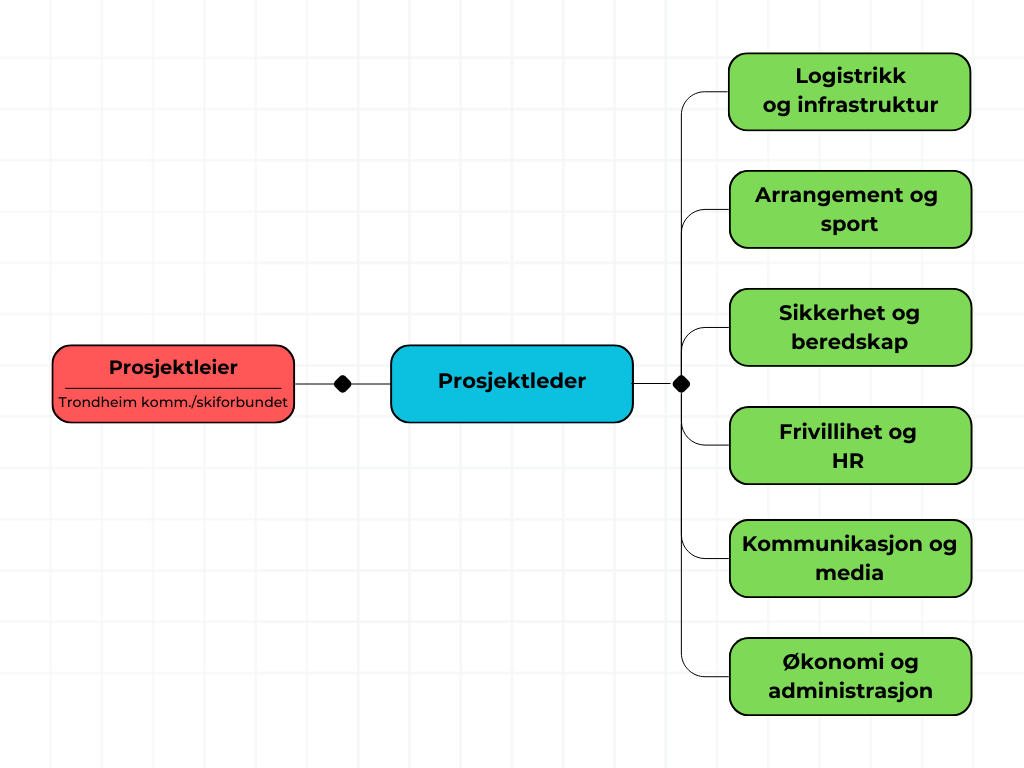
\includegraphics[width=10cm]{organisasjonskart}
    \caption{Organisasjonskart}
    \label{fig:organisasjonskart}
\end{figure}